\begin{frameO}[We want]

    A \emph{lot} of IoT devices 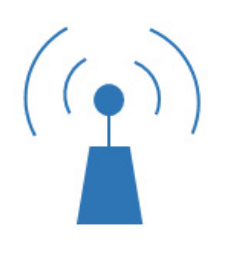
\includegraphics[height=0.37cm]{dynamic-devices.png} want to access to \emph{one} gateway
    % (base station).

    \begin{itemize}
        % \tightlist
        \item
            Insert them in an already \textbf{crowded wireless network}
        \item
            With a protocol \textbf{slotted in time and frequency}
        \item
            Each device 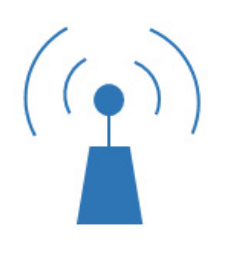
\includegraphics[height=0.37cm]{dynamic-devices.png} / 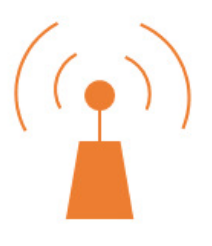
\includegraphics[height=0.37cm]{static-devices.png} has a \textbf{low duty cycle} \hfill{}
            \textcolor{gray}{ex: few messages per day}
    \end{itemize}

    \pause

    \only<1-2>{
        % \begin{figure}[!h]
        \centering
        \includegraphics[width=0.70\linewidth]{system_model1.eps}
        % \caption{In our system model, some dynamic devices (in the \textcolor{blue}{IoT network in blue}) transmit packets to a gateway and suffer from the interference generated by neighboring networks (in \textcolor{orange}{orange left/right}).}
        % \label{fig:41:system_model1}
        % \end{figure}
    }

    % \only<3>{
    %     % \pause

    %     \begin{colorblock}{Goal}
    %         \begin{itemize}
    %             % \tightlist
    %             \item Maintain a \textbf{good Quality of Service}.
    %             \item \textbf{Without} centralized supervision!
    %         \end{itemize}
    %     \end{colorblock}

    %     % \pause

    %     \begin{alertblock}{How?}
    %         \begin{itemize}
    %             % \tightlist
    %             \item Use \textbf{learning algorithms}\newline
    %             $\implies$ can devices learn on which frequency they should talk ?
    %         \end{itemize}
    %     \end{alertblock}
    % }

\end{frameO}



\subsection{Model and hypotheses}

\subsubsection{A new model for IoT networks}

\begin{frameO}[A new model for IoT networks]

    \begin{itemize}
        % \tightlist
        \item
              Discrete time \(t\geq1\) and \(K\) radio channels (\emph{e.g.}, 10)
              \hfill{} (\emph{known})
    \end{itemize}

    \begin{figure}[h!]
        \centering
        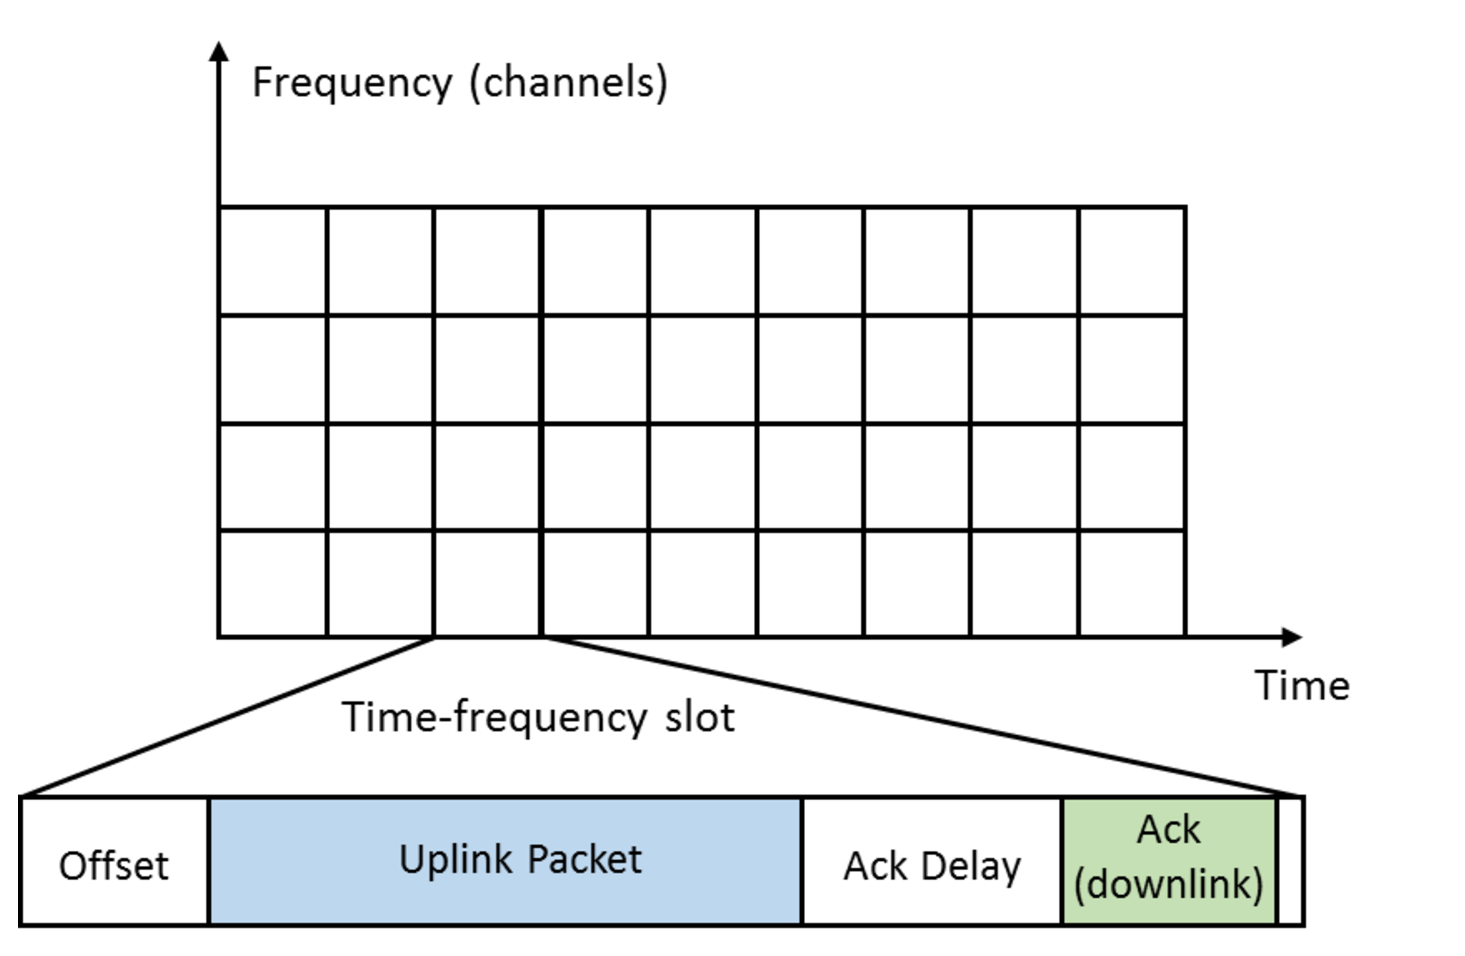
\includegraphics[height=0.35\textheight]{protocol.eps}\\
        
        {\small Chosen protocol: \textcolor{blue}{uplink messages {\large $\nearrow$}} followed by \textcolor{darkgreen}{\emph{acknowledgements} {\large $\searrow$}}}\\
        \hfill{} {\tiny \textcolor{gray}{[Bonnefoi, Besson et al, CROWNCOM 2017], Sec.5.2}}
    \end{figure}

    \begin{itemize}
        % \tightlist
        \item
              \(D\) \textbf{dynamic} devices 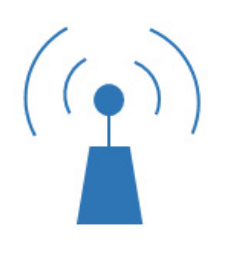
\includegraphics[height=0.37cm]{dynamic-devices.png} trying to access the network \emph{independently}
        \item
              \(S=S_1+\dots+S_{K}\) \textbf{static} devices 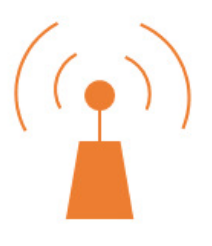
\includegraphics[height=0.37cm]{static-devices.png} occupying the network:
              \newline
              \(S_1,\dots,S_{K}\) in each channel \(\{1,\dots,K\}\) \hfill{} (\emph{unknown})
    \end{itemize}

\end{frameO}


\begin{frameO}[Protocol: \textcolor{blue}{uplink messages {\large $\nearrow$}} followed by \textcolor{darkgreen}{\emph{acknowledgements} {\large $\searrow$}}]

    \begin{center}
        \only<1>{
            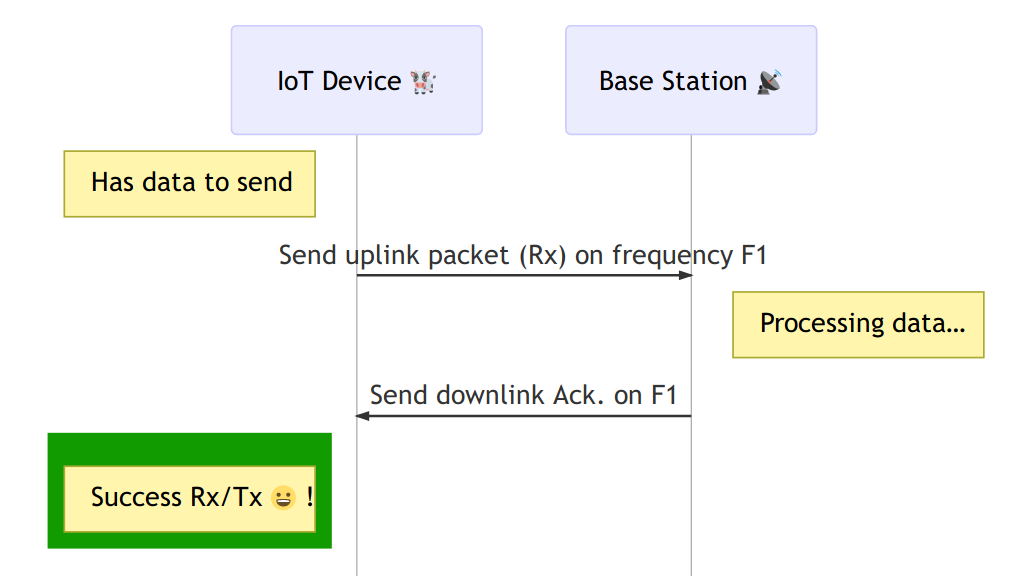
\includegraphics[width=0.90\textwidth]{Protocol_successful_transmission.png}
            \underline{1st case}: Successful transmission if no collision on \textcolor{blue}{uplink messages {\large $\nearrow$}} !
        }
        \only<2>{
            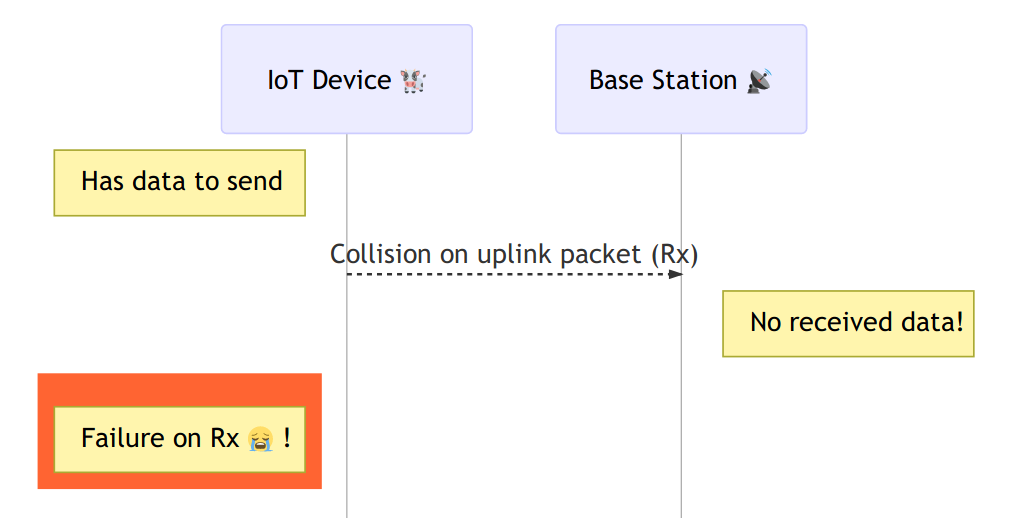
\includegraphics[width=0.90\textwidth]{Protocol_failed_transmission.png}
            \underline{2nd case}: Failed transmission if collision on \textcolor{blue}{uplink messages {\large $\nearrow$}}
        }
    \end{center}

\end{frameO}


\subsubsection{Hypotheses}

\begin{frameO}[Our model of IoT devices \hfill{} \textcolor{gray}{[Bonnefoi, 2017]}]

    \begin{lightblock}{Emission model for static and dynamic devices}

        \begin{itemize}
            % \tightlist
            \item
                Each device 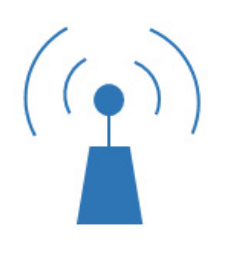
\includegraphics[height=0.37cm]{dynamic-devices.png} / 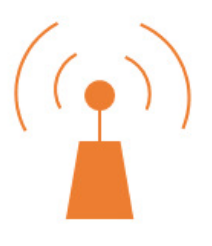
\includegraphics[height=0.37cm]{static-devices.png}  has the same \emph{low} emission probability: \\
                each step, each device sends a packet with probability \(p\)
                %   \\
                %   \hfill{}\small{(this gives a duty cycle proportional to $1/p$)}
        \end{itemize}

    \end{lightblock}

    \vspace*{5pt}
    \pause
    \begin{colorblock}{Background \textbf{stationary} ambiant traffic}

        \begin{itemize}
            % \tightlist
            \item
                  Each static device 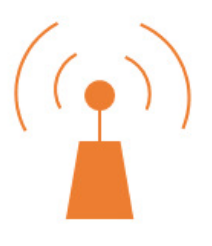
\includegraphics[height=0.37cm]{static-devices.png} uses only one channel
            \item
                  Their repartition is fixed in time
                  % \hfill{} $\implies$ \alert{stationary} hypothesis!
        \end{itemize}

        \(\implies\) This (stationary) ambiant traffic \emph{is disturbing} the dynamic devices 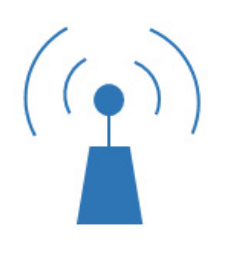
\includegraphics[height=0.37cm]{dynamic-devices.png}
    \end{colorblock}

    \vspace*{5pt}
    \pause
    \begin{colorblock}{Dynamic radio reconfiguration}

        \begin{itemize}
            % \tightlist
            \item
                \textbf{Dynamic device decide} 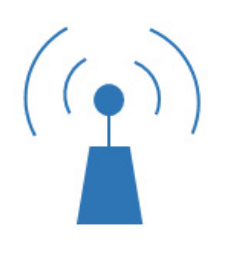
\includegraphics[height=0.37cm]{dynamic-devices.png}  the channel to use to send their packets
            \item
                They all have memory and computational capacity to implement small decision algorithms
                % on a small CPU embedded on the devices.
        \end{itemize}

    \end{colorblock}

\end{frameO}


\begin{frameO}[Problem]

    \begin{lightblock}{Goal}
        \emph{minimize packet loss ratio} (max \(=\) number of received \texttt{Ack})\\
        in a \emph{finite-space discrete-time Decision Making Problem}
    \end{lightblock}

    \vspace*{20pt}

    \begin{lightblock}{Baseline (naive solution)}
        Purely random (uniform) spectrum access for each of the $D$ dynamic devices 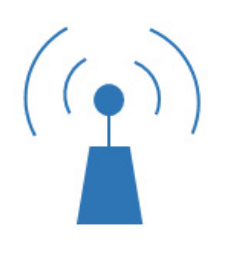
\includegraphics[height=0.37cm]{dynamic-devices.png} .
    \end{lightblock}

    \begin{lightblock}{A possible solution}
        Embed a \textbf{decentralized Multi-Armed Bandit} algorithm, running \textbf{independently on each dynamic device} 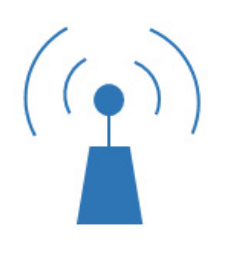
\includegraphics[height=0.37cm]{dynamic-devices.png}
    \end{lightblock}

\end{frameO}



\subsection{Baseline algorithms}

% \subsubsection{$1)$ A naive strategy: uniformly random access}

% \begin{frameO}[$1)$ A naive strategy: uniformly random access]

%     \begin{itemize}
%         % \tightlist
%         \item
%               \textbf{Uniformly random access}: dynamic devices choose uniformly
%               their channel in the pull of \(K\) channels.
%         \item
%               Natural strategy, dead simple to implement.
%     \end{itemize}

%     \pause

%     \begin{itemize}
%         % \tightlist
%         \item
%             Simple analysis, in term of \textbf{successful transmission
%             probability}\newline
%             (for every message from dynamic devices):
%     \end{itemize}

%     \begin{small} \begin{align*}
%             \mathbb{P}(\text{success}|\text{sent}) = \sum_{k=1}^{K} \underbrace{(1 - p / K)^{D-1}}_{\text{No other dynamic device}} \times \underbrace{(1-p)^{S_k}}_{\text{No static device}} \times\; \frac{1}{K}.
%         \end{align*} \end{small}

%     \pause

%     \begin{itemize}
%         % \tightlist
%         \item
%               Works fine only if all channels are similarly occupied,\newline
%               but \textbf{it cannot learn} to exploit the best (more free)
%               channels.
%     \end{itemize}

% \end{frameO}



\subsubsection{$1)$ \emph{Oracle} centralized strategy}

\begin{frameO}[$1)$ \emph{Oracle} centralized strategy \hfill{} \textcolor{gray}{[Bonnefoi, 2017]}]

    \begin{itemize}
        % \tightlist
        \item
              If an oracle can affect \(D_k\) dynamic devices 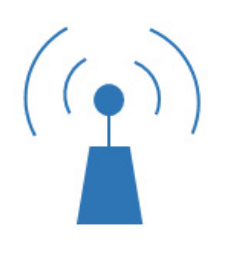
\includegraphics[height=0.37cm]{dynamic-devices.png}  to channel
              \(k\) \slotmachine{}, the \textbf{successful transmission probability} of the entire network is
              \vspace*{-10pt}

              \begin{small} \begin{align*}
                      \mathbb{P}(\text{success}|\text{sent}) = \sum_{k=1}^{K} \underbrace{(1 - p)^{D_k - 1}}_{\;\;D_k - 1 \;\text{others}\;\;} \times \underbrace{(1 - p)^{S_k}}_{\;\;\text{No static device}\;\;} \times \underbrace{ D_k / D }_{\;\;\text{Sent in channel}\; k}
                  \end{align*} \end{small}
              \pause
        \item
              The oracle has to solve this \textbf{optimization problem}:
              \vspace*{-5pt}

              \begin{small} \begin{equation*} \begin{cases}
                          \underset{D_1,\dots,D_{K}}{\arg\max}\;\;\; & \sum\limits_{k=1}^{K} D_k (1 - p)^{S_k + D_k -1}                                           \\
                          \text{such that}\;\;\;                     & \sum\limits_{k=1}^{K} D_k = D \; \text{and} \; D_k \geq 0, \; \; \forall 1 \leq k \leq K .
                      \end{cases} \end{equation*} \end{small}
        \item
              \textcolor{orange}{Contribution}: we solved this quasi-convex optimization problem with \emph{Lagrange
                  multipliers} (only numerically).
    \end{itemize}

    \vfill{}
    \begin{colorblock}{}
        \(\implies\) It will have very good performance, as it maximizes the transmission rate of all the \(D\) dynamic devices
        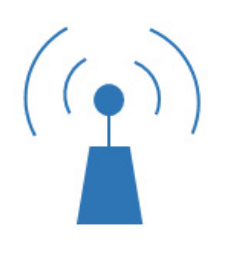
\includegraphics[height=0.37cm]{dynamic-devices.png}
    \end{colorblock}

\end{frameO}

\begin{frameO}[$1)$ \emph{Oracle} centralized strategy]

    \begin{colorblock}{But unrealistic}
        But \textbf{not achievable in practice}!
        \begin{itemize}
            % \item
            % there is no oracle
            \item \alert{because there is no centralized supervision!}
        \end{itemize}
    \end{colorblock}

    \vspace*{30pt}

    \begin{colorblock}{Let see \emph{realistic decentralized approaches}}

        \(\hookrightarrow\) Machine Learning \newline
        \hspace*{15pt}\(\hookrightarrow\) Reinforcement Learning \newline
        \hspace*{30pt} \(\hookrightarrow\) \emph{Multi-Armed Bandit}

    \end{colorblock}

\end{frameO}



\begin{frameO}[Hum, what is a (one-armed )\emph{bandit}?]
    \begin{center}
        It's an old name for a casino machine \slotmachine{} !
    \end{center}

    \begin{center}
        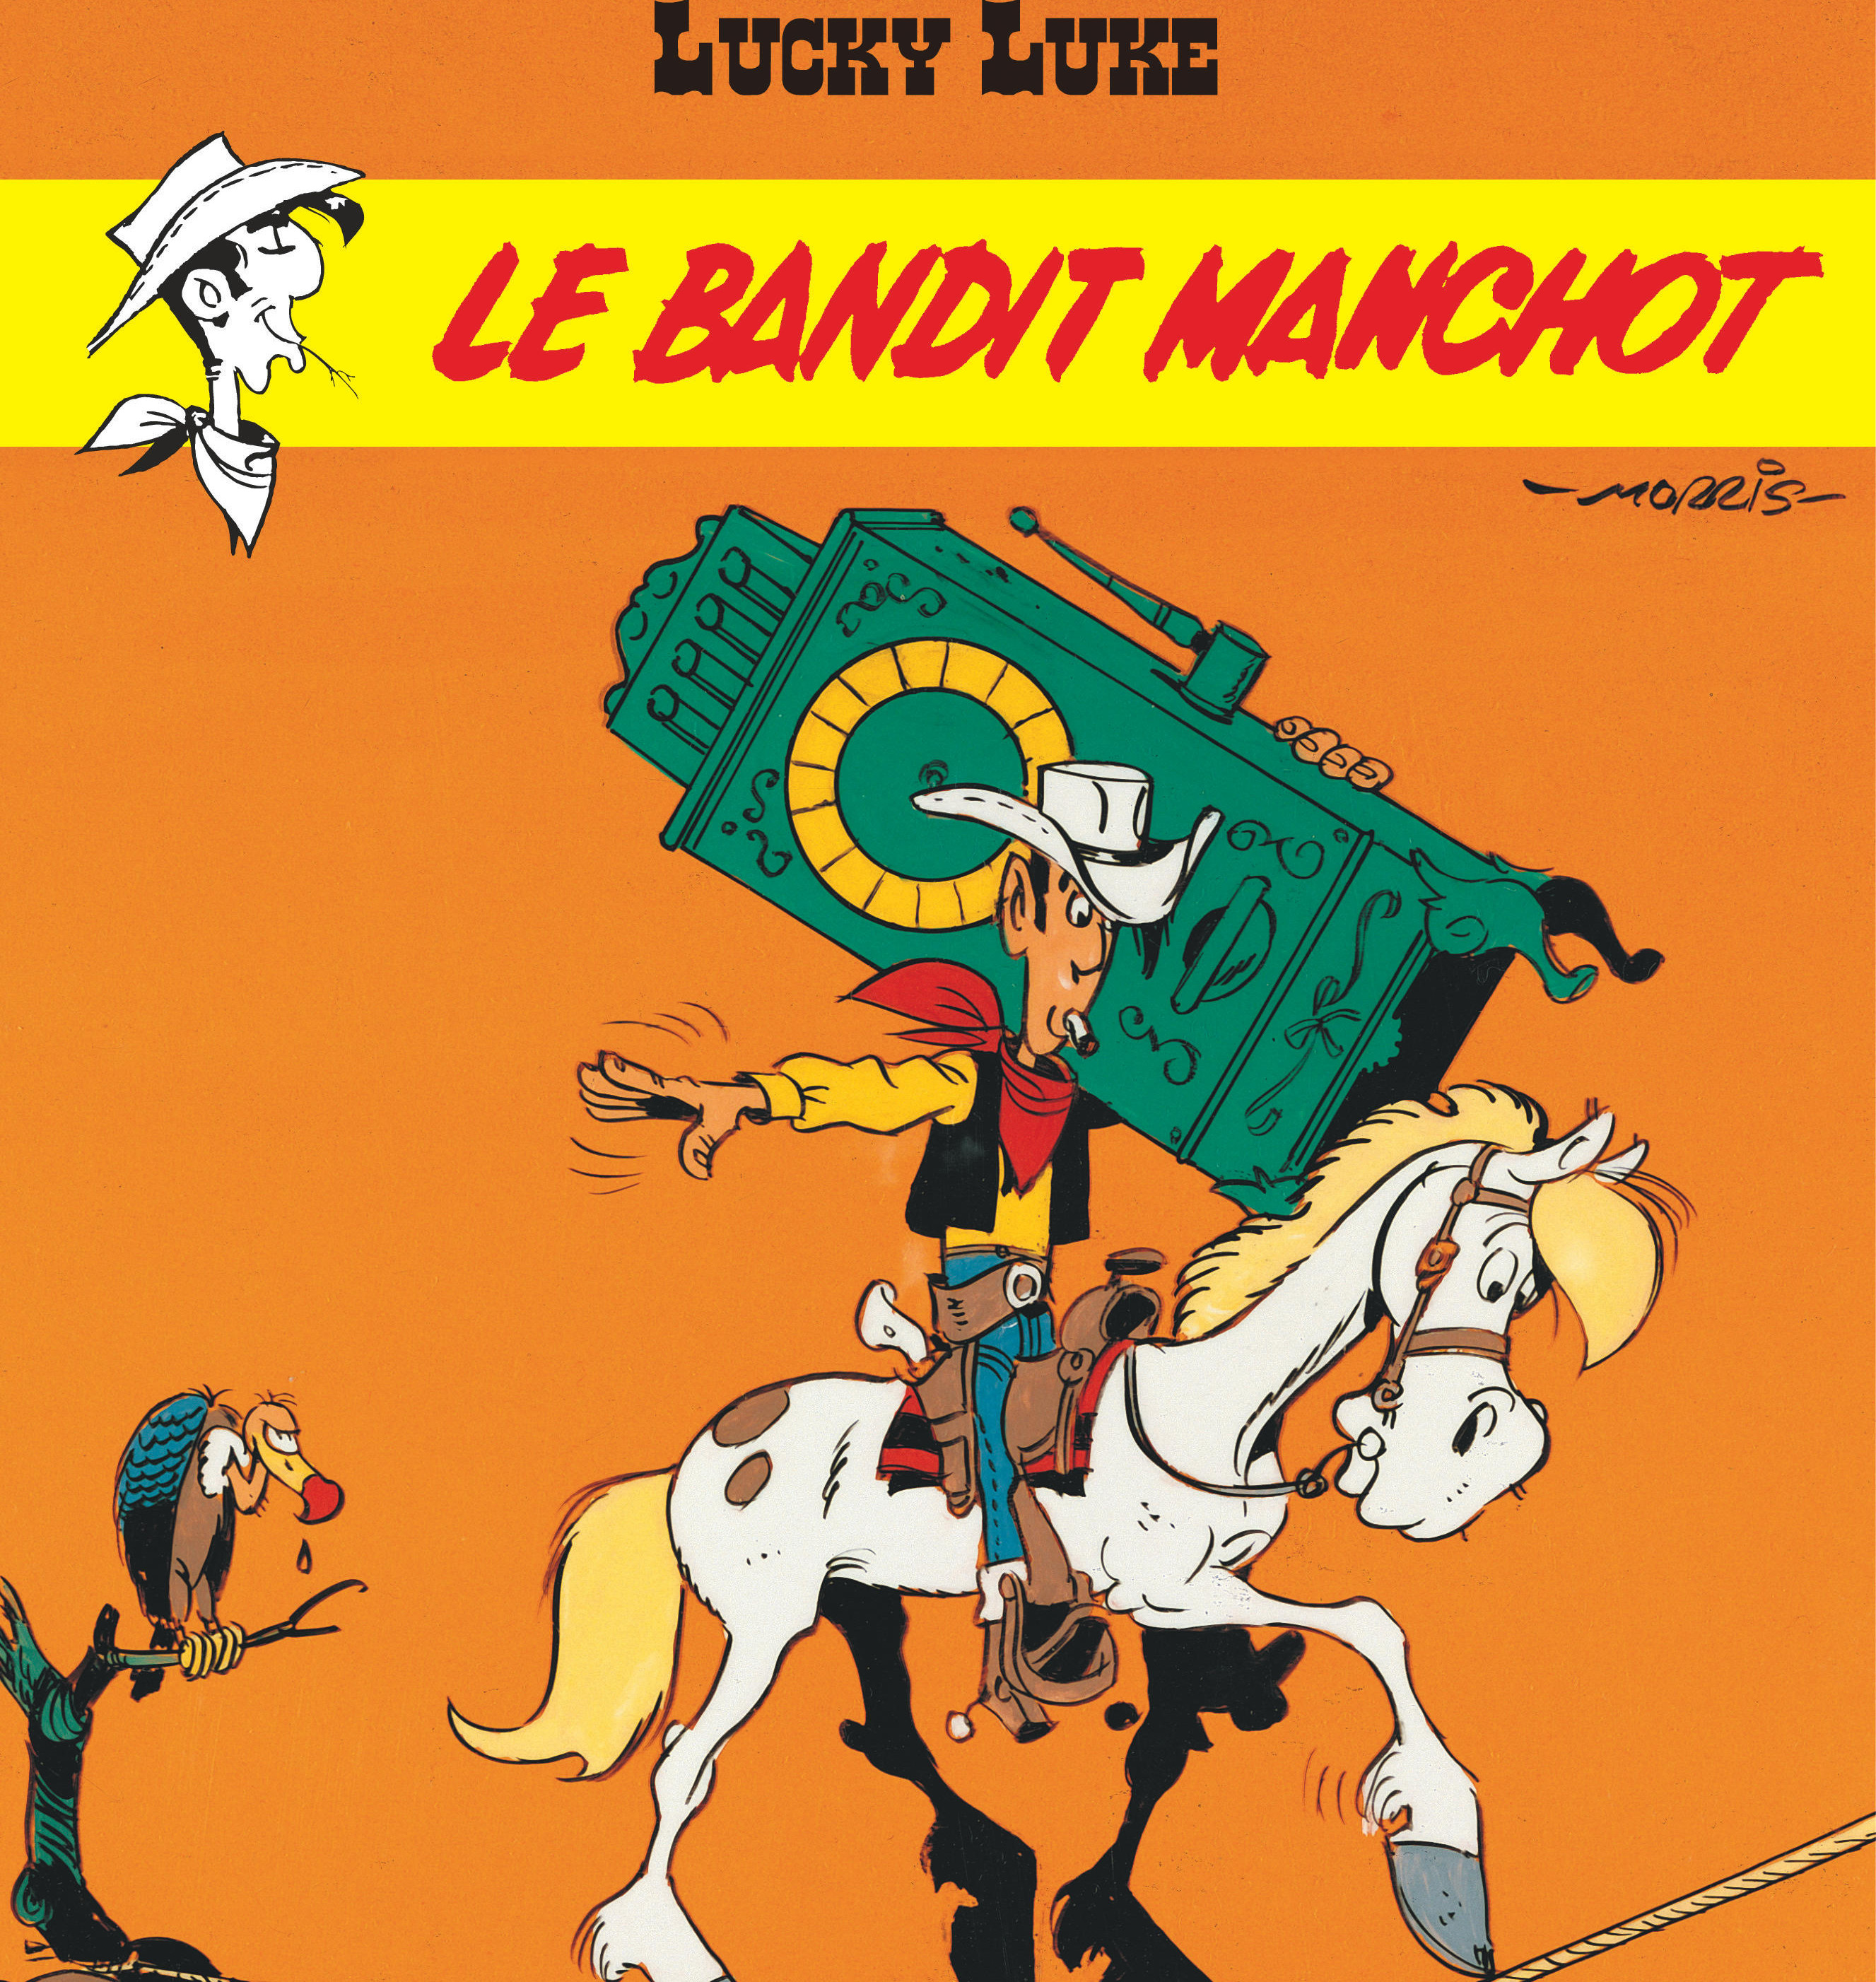
\includegraphics[height=6.5cm]{Lucky_Luke__Le_Bandit_Manchot.jpg}

        \begin{tiny}
            \textcolor{gray}{
                \textcopyright{} Dargaud,
                \href{https://www.dargaud.com/bd/LUCKY-LUKE/Lucky-Luke/Lucky-Luke-tome-18-Bandit-manchot-Le}{\textcolor{blue}{Lucky Luke tome 18}}.
            }
        \end{tiny}
    \end{center}
\end{frameO}



\subsection{Multi-Armed Bandit algorithm: UCB}

\subsubsection{Multi-Armed Bandit formulation}

\begin{frameO}[Stochastic \emph{Multi-Armed Bandit} formulation]

    A player tries to collect \emph{rewards} when playing a $K$-armed \slotmachine{} bandit game.

    \begin{lightblock}{}
        At each time step $t\in\{1,\dots,T\}$
        \begin{itemize}
            % \tightlist
            \item
                player chooses an \emph{arm} \slotmachine{} \(A(t) \in \{1,\dots,K\}\)
            \item
                the arm generates an i.i.d. \emph{reward} $r_{A(t)}(t) \sim \nu_{A(t)}$\\
                \textcolor{gray}{Ex: from a Bernoulli distribution $\nu_{k} = \mathcal{B}(\mu_k)$}
            \item
                player observes the reward $r_{A(t)}(t)$
        \end{itemize}
    \end{lightblock}

    \pause

    \begin{colorblock}{Goal}
        Maximize the sum reward (\textbf{Reinforcement Learning}) or \textcolor{orange}{its expectation}
        \[\max_{A} \;\; \sum\limits_{t=1}^{T} r_{A(t)} \,\,\,\,\,\, \text{or} \,\,\,\,\,\, max_{A} \;\; \textcolor{orange}{ \mathbb{E}[\sum\limits_{t=1}^{T} r_{A(t)}] }.\]
    \end{colorblock}

    \vfill{}
    \hfill{} {\tiny \textcolor{gray}{[Bubeck, 2012], [Lattimore \& Szepesvári, 2019], [Slivkins, 2019]}

\end{frameO}

\begin{frameO}[$2)$ Pseudo \emph{MAB} formulation of our IoT problem]

    A dynamic device 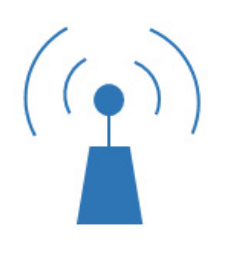
\includegraphics[height=0.37cm]{dynamic-devices.png}  tries to collect \emph{rewards} when transmitting:

    \begin{itemize}
        % \tightlist
        \item
            it transmits following a random Bernoulli process \newline
            (of probability \(p\) of transmitting at each time step \(t\)),
        \item
            it chooses a channel \(A(\tau) \in \{1,\dots,K\}\)
            \hfill{} ($=$ arm \slotmachine)
        \begin{itemize}
        \item
            if \texttt{Ack} (no collision) \hspace*{2pt} \(\implies\) reward
            \(r_{A(\tau)} = 1\) \hfill{} (successful transm.!)
        \item
            if collision (no \texttt{Ack}) \hspace*{2pt} \(\implies\) reward
            \(r_{A(\tau)} = 0\) \hfill{} (failed transmission!)
        \end{itemize}

    \end{itemize}

    \pause

    \begin{colorblock}{Goal}
        Maximize transmission rate \(\equiv\) \textbf{maximize cumulated rewards}
        % \(\equiv \max_{A} \;\; \sum\limits_{\tau=1}^{\text{nb of transm.}} r_{A(\tau)}\).
    \end{colorblock}

    \begin{lightblock}{It is not a \emph{stochastic} Multi-Armed Bandit problem}
        \textcolor{orange}{It looks like a MAB}
        but the \textbf{environment is not stochastic or stationary}
        % \newline
        % {\small (if only one device is activated at a time: average reward \(\mathbb{E}[r_k(\tau)] = p S_k\))}
    \end{lightblock}

\end{frameO}

\subsubsection{Upper Confidence Bound algorithm: UCB}

\begin{frameO}[$2)$ Upper Confidence Bound algorithm (\(\mathrm{UCB}_1\))]

    \only<1-2>{
        A dynamic device keeps \(\tau\) number of sent packets
    }

    \begin{enumerate}
        \def\labelenumi{\arabic{enumi}.}

        % \tightlist
        \only<1-2>{
            \item
              For the first \(K\) activations (\(\tau=1,\dots,K\)), try each channel
              \emph{once}.
        }
        \pause
        \item
              Then for the next steps \(t\):

              \begin{itemize}
                  % \tightlist
                  \item
                        \textcolor{orange}{With probability $p$, the device is active ($\tau := \tau + 1$)}
                \only<1-2>{
                  \item
                        Compute the index
                        \(\mathrm{UCB}_k(\tau) := \overbrace{\frac{X_k(\tau)}{N_k(\tau)}}^{\text{Mean}\; \widehat{\mu_k}(\tau)} + \overbrace{\sqrt{\frac{\log(\tau)}{2 N_k(\tau)}},}^{\text{Confidence Bonus}}\)
                  \item
                        Choose channel
                        \(A(\tau) = \mathop{\arg\max}\limits_{k} \; \mathrm{UCB}_k(\tau)\),
                  \item  Observe reward $r_{A(\tau)}(\tau)$ from arm $A(\tau)$
                  \begin{itemize}
                  \item
                        Update \(N_k(\tau+1)\) nb selections of channel \(k\)
                        % \newline
                        % \(N_{A(\tau)}(\tau+1) = N_{A(\tau)}(\tau) + 1\) else
                        % \(N_k(\tau+1) = N_k(\tau)\)
                    \item
                        Update \(X_k(\tau)\) nb of successful transmissions
                        % \newline
                        % \(X_{A(\tau)}(\tau+1) = X_{A(\tau)}(\tau) + r_{A(\tau)}(\tau)\) else
                        % \(X_k(\tau+1) = X_k(\tau)\)
                  \end{itemize}
                }
                \only<3>{
                    \item Play UCB algorithm\dots{}
                }
                  \item
                        \textcolor{orange}{Wait for next message\dots \hfill{} (mean waiting time $\simeq 1/p$)}
              \end{itemize}
    \end{enumerate}

    \only<1-2>{
        \hfill{}
        {\small \textcolor{gray}{Ref: [Auer et al, 2002]}}
    }
    \only<3>{
    \begin{colorblock}{Multiple devices}
        The collisions are not stochastic!
    \end{colorblock}
    \begin{colorblock}{Random activation times $\tau$?}
        \begin{itemize}
            \item
                  The times $\tau$ are \textbf{not} the global time indexes $t$
            \item
                  each object transmits only with probability $p$ at each time $t$\newline
                  (following its Bernoulli activation pattern)
        \end{itemize}
    \end{colorblock}
    \vspace*{10pt}
        {\large
            \alert{$\implies$ these two problems make the model \textbf{hard to analyze} !}
        }
    }

    % \vfill{}\hfill{}\tiny{\textcolor{gray}{References: [Lai \& Robbins, 1985], [Auer et al, 2002], [Bubeck \& Cesa-Bianchi, 2012]}}

\end{frameO}



\subsection{Experimental results}

\subsubsection{Experiment setting}

\begin{frameO}[Experimental setting: simulation parameters]

    % \begin{colorblock}{}

        \begin{itemize}
            % \setlength\itemsep{10pt}
                  % 
                  % \tightlist
            \item
                  \(K = 10\) channels \slotmachine,
            \item
                  \(S\) 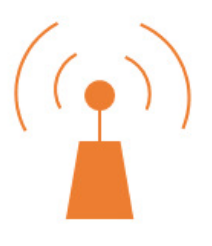
\includegraphics[height=0.37cm]{static-devices.png}
                  \(+\)
                  \(D\) 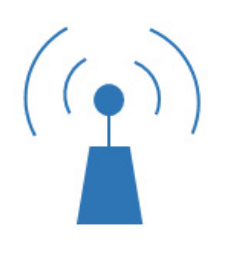
\includegraphics[height=0.37cm]{dynamic-devices.png}
                  \(= 10000\) devices
                  in total,
            \pause
            \item
                  \(p = 10^{-3}\) probability of emission,
            \item
                  Horizon \(T = 10^5\) total time slots
                  (\textcolor{orange}{avg. \(\simeq 100\) messages \(/\) device}),
            \pause
            \item
                  We change the proportion of dynamic devices
                  \(D\)
                  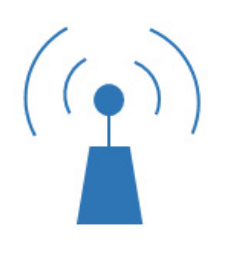
\includegraphics[height=0.37cm]{dynamic-devices.png}
                  \(/\)
                  \((S\)
                  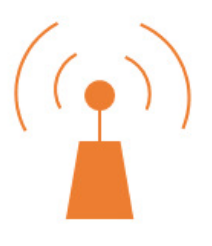
\includegraphics[height=0.37cm]{static-devices.png}
                  \(+\)
                  \(D\)
                  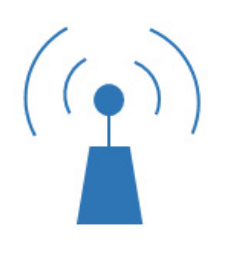
\includegraphics[height=0.37cm]{dynamic-devices.png}
                  \()\),
            \item
                  For one example of repartition of \((S_1,\dots,S_{K})\) static devices 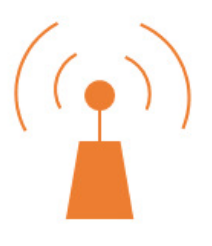
\includegraphics[height=0.37cm]{static-devices.png}
        \end{itemize}
        \vspace*{-10pt}
        \begin{center}
            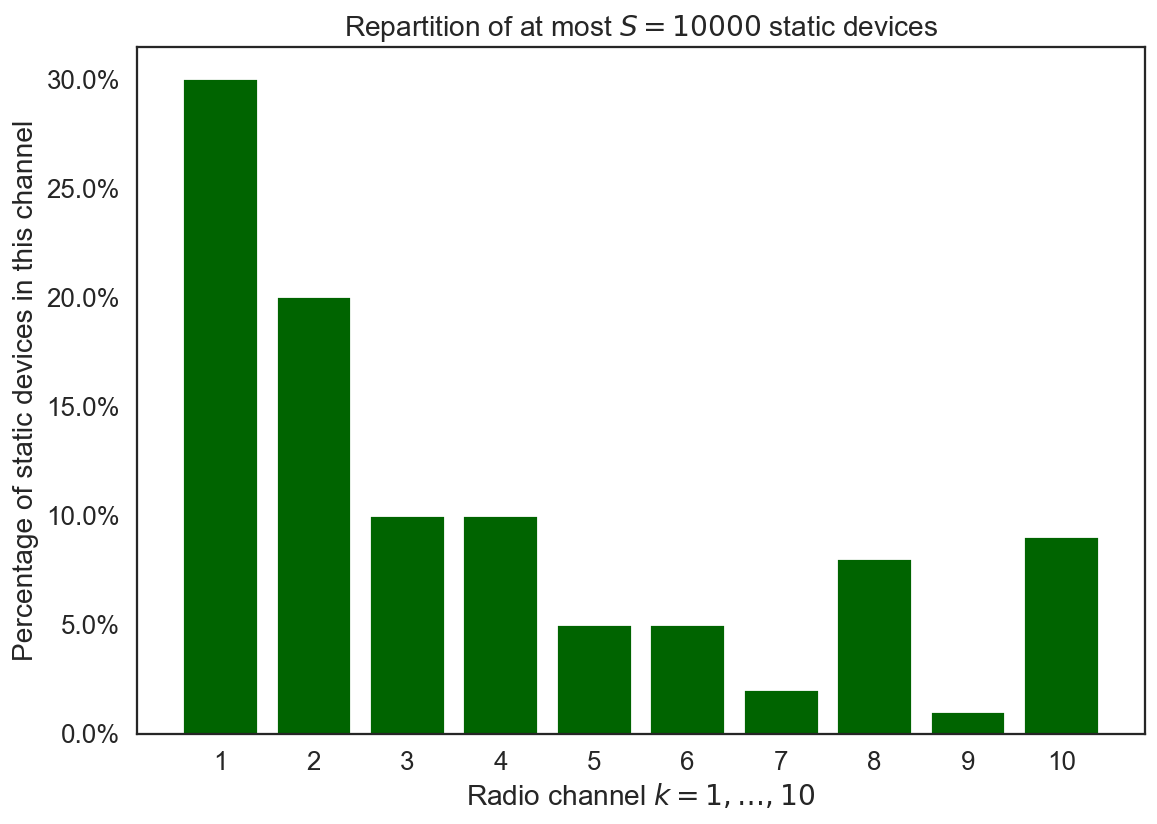
\includegraphics[height=3.5cm]{Repartition_of_static_devices.png}
        \end{center}

    % \end{colorblock}

\end{frameO}



\subsubsection{First result: $10\%$}

\begin{frameO}[\(10\%\) of dynamic devices]

    \begin{figure}[h!]
        \centering
        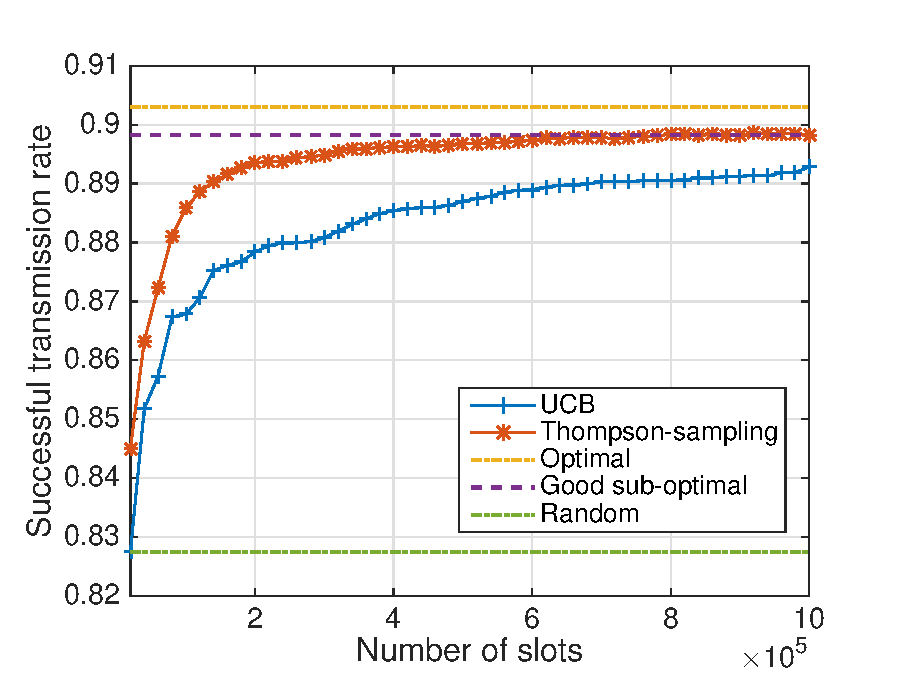
\includegraphics[height=0.74\textheight]{10intelligent.eps}

        % \caption{
            $10\%$ of dynamic devices 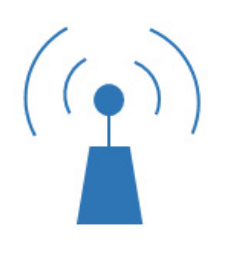
\includegraphics[height=0.37cm]{dynamic-devices.png}. Gives $7\%$ of gain.\\
            {\small \textcolor{gray}{[Bonnefoi, Besson et al, CROWNCOM 2017], Sec.5.2}}
        % }
    \end{figure}

\end{frameO}



% \subsubsection{Second result: $30\%$}

% \begin{frameO}[\(30\%\) of dynamic devices]

%     \begin{figure}[h!]
%         \centering
%         \includegraphics[height=0.74\textheight]{30intelligent.eps}

%         % \caption{
%             \begin{small}
%                 $30\%$ of dynamic devices 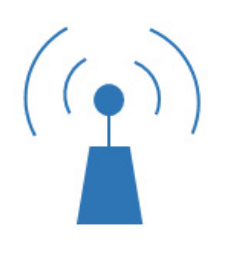
\includegraphics[height=0.33cm]{dynamic-devices.png}. Gives $3\%$ of gain but not much is possible here.
%             \end{small}
%         % }
%     \end{figure}

% \end{frameO}


\subsubsection{Growing proportion of devices dynamic devices}

\begin{frameO}[Dependency on \(D/(S+D)\)]

    \begin{figure}[h!]
        \centering
        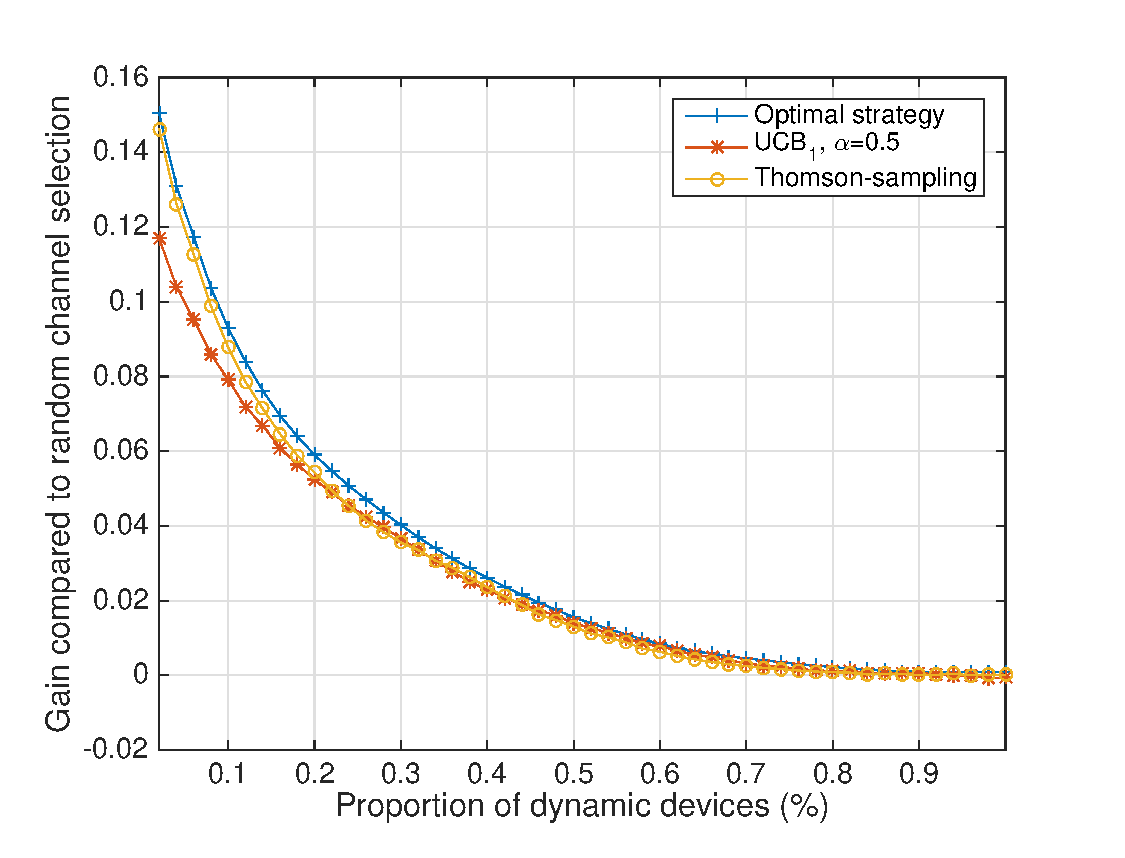
\includegraphics[height=0.70\textheight]{perf_learning.eps}

        % \caption{
            \emph{Almost optimal}, for any proportion of dynamic devices 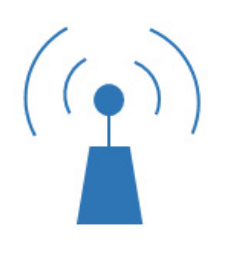
\includegraphics[height=0.37cm]{dynamic-devices.png}, \emph{after a short learning time}. Up-to $16\%$ gain over the naive approach!
        % }
    \end{figure}

\end{frameO}


% \begin{frameO}[\emph{Positive} conclusion from experiments ($1/2$)]

%     \begin{colorblock}{What do we show}

%         \begin{itemize}
%             \setlength\itemsep{10pt}
%                   % \tightlist
%             \item
%                   After a short learning time, MAB algorithms are almost as efficient as
%                   the oracle solution,
%             \item
%                   Never worse than the naive solution, even at first iterations,
%             \item
%                   Thompson sampling is more efficient than UCB
%                   (as always),
%             \item
%                   The dynamic devices 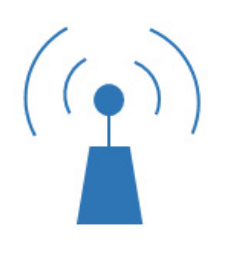
\includegraphics[height=0.37cm]{dynamic-devices.png} can learn to communicate more efficiently,\\
%                   in any network configuration (we tried a lot more!).
%         \end{itemize}

%     \end{colorblock}

% \end{frameO}


% \begin{frameO}[\emph{Negative} conclusion from experiments ($2/2$)]

%     \begin{lightblock}{But what are the limitations?}

%         \begin{itemize}
%             \setlength\itemsep{5pt}
%                   % \tightlist
%             \item
%                 \textcolor{orange}{\textbf{Only works empirically}!}
%                 \\
%                 Theoretically, we showed counter examples where the \textbf{Selfish} approach can fail, for the smallest case $D = 2$ devices, $p=1$ in $K=3$ channels
%             \item
%                 $p \times (D + S)$ devices in $K$ channels in average\\
%                 $\implies$ $p \ll \frac{K}{(D + S)}$ gives best performance
%             \item
%                 Only works empirically with a stationary hypothesis on the background traffic\dots
%             \item
%                 \textbf{Intractable model} in theory, mainly due to too much randomness (activations, collisions, selections\dots)
%         \end{itemize}

%     \end{lightblock}

% \end{frameO}
